\documentstyle[12pt,doctor,xbmkanji,epsf, graphicx,float,url,multirow]{master}
% \documentstyle[12pt,doctor,xbmkanji,eclepsf]{mybook}
% \documentstyle[12pt,doctor,gaij,epsbox]{mybook}
\addtolength{\headsep}{1cm}
\addtolength{\topmargin}{-2cm}
\addtolength{\textheight}{2cm}

% 以前はこうなってました
% \addtolength{\oddsidemargin}{0.2cm}
% \addtolength{\evensidemargin}{-2.35cm}
% \addtolength{\textwidth}{2cm}

% 指定された左2.5cm 右1.5cmぐらいの余白になる
\addtolength{\oddsidemargin}{-1.0cm}
\addtolength{\evensidemargin}{-3.6cm}
\addtolength{\textwidth}{5.5cm}

\begin{document}

%
% 表紙
%
%近畿大学理工学部情報学科卒業研究報告書表紙
% ver 0.1 2005/11/28 by Toru Kato
% ver 0.2 2006/11/28 by Takashi Ishimizu
% ver 0.3 2008/11/26 by Toru Kato
% ver 0.4 2009/12/14 by Shoji Mizobuchi
\begin{titlepage}
\begin{center}
\LARGE
\vspace*{1cm}

\Huge{修\hspace{2zw}士\hspace{2zw}論\hspace{2zw}文}\\
\vspace{1cm}
\huge{令和四年度}\\

\vspace*{9cm}
\vspace*{2cm}
\huge{近畿大学大学院\\
総合理工学研究科\\
エレクトロニクス系工学専攻\\
21-3-334-0415番 \hspace{0.5zw} 栗\hspace{0.5zw}岡\hspace{0.5zw}陽\hspace{0.5zw}平
}
\end{center}
\end{titlepage}
 

%%% Local Variables: 
%%% mode: latex
%%% TeX-master: t
%%% End: 


%
% 概要
%
\begin{titlepage}
\begin{center}
\vspace*{1cm}
\Large
{\Huge 修\hspace{2zw}士\hspace{2zw}論\hspace{2zw}文}\\
\vspace*{1cm}
{\huge 令和五年度}\\
\vspace*{2cm}
{\huge 論文内容の要旨}\\
\vspace*{1cm}
{\LARGE グラフデータベースを用いた\\
学習者理解度可視化システムの開発
}\\
\vspace*{7cm}
\LARGE{近畿大学大学院\\
総合理工学研究科\\
エレクトロニクス系工学専攻\\
21-3-334-0415番 \hspace{0.5zw} 栗\hspace{0.5zw}岡\hspace{0.5zw}陽\hspace{0.5zw}平
}
\end{center}
\end{titlepage}

\newpage

\begin{titlepage}

    %背景
    2019 年 12 月に文部科学省が作成した「教育の情報化に関する手引き」\cite{tebiki}によると教育の情報化が促進されている.
    e ラーニング\cite{e}は「情報通信技術の時間的・空間的制約をなくす」,「双方向性を有する」,「カスタマイズを容易にする」という特性を有するシステムのうちの一つであることから,教育の情報化に有効である.
    e ラーニング上で学習するにあたり,自身の学習目標を設定することは,学びを深める手段のうちの一つである\cite{seman}.
    一方,学習目標を設定するには,自身が学習したい対象の知識を把握している必要がある.
    しかし,学習者自身では学習項目を理解していると主観的には考えていても,他人が客観的に判断すると理解できていない場合があり,学習者自身で学習目標を設定することは必ずしも容易ではない.

    %関連研究
    東本氏らの研究では,科学領域においては習得すべきさまざまな概念および概念間の関係が存在し,その一つに概念の階層構造を学習者に理解させることは科学の学習において重要な課題であると認識していた.
    そこで,階層構造の理解の促進を目的とした学習者自身によるコンセプトマップ(以下,CMap)\cite{concept}の構築のためのシステムを開発した\cite{toumoto}.
    野村氏らの研究では,学習方法の一つとして,学習した内容を整理して他の学習者に教える事で自信の理解を深める方法があり,
    他者に対して学習内容を理解させることができるか否かで自身の理解が十分であるか否かを学習者自身が再確認することができるという教え合い学習をシステムの推奨を用いて実際に学習者間で行わさせることを目的とした研究を進めている.\cite{nomura}

    %本研究
    そこで本研究では,学習目標の設定支援を目的に,学習者の理解度を可視化する,グラフデータベース を用いた学習者理解度可視化システムを開発した.
    本システムは e ラーニングで学習している学習者を対象としたシステムで,CMapを利用して学習者が学習目標を設定する場合に本システムを利用することを想定している.
    学習者は指導者が作成した問題を解き,本システムを用いて CMap を作成する.
    本システムでは学習者の回答情報から CMapを作成し,学習者は自身が作成した CMap と,システムが生成した CMap を比較することにより,自身の学習理解度を客観的に確認でき,学習目標設定の基準にできる.
    
    %実験
    
\end{titlepage}

%
% 内表紙
%

%%%%%%%%%%%%%%%% 内表紙 %%%%%%%%%%%%%%%

\begin{titlepage}
    \begin{center}
    \vspace*{3cm}
    \large
    {\Huge 修\hspace{2zw}士\hspace{2zw}論\hspace{2zw}文}\\
    \vspace*{3cm}
    {\LARGE グラフデータベースを用いた\\学習者理解度可視化システムの開発}
    \\
    \vspace*{1cm}
    {\large Development of a Visualization System for Learner Comprehension \\ Using a Graph Database}
    \end{center}
\end{titlepage}

\setlength{\baselineskip}{1.2\baselineskip}

%%% 目次 %%%
\pagestyle{plain}
\pagenumbering{roman}
\addcontentsline{toc}{section}{目次}
\tableofcontents

%%%%% 行頭文字下げの設定 %%%%%

\parindent=1em

\clearpage
\pagestyle{headings}
\pagenumbering{arabic}

%
% 序論
%
\chapter{はじめに}
\label{chap:introduction}
\section{本章の概要}
本章では,研究背景と研究目的,評価実験の概要,そして本論文の構成について記載する.

研究背景では,教育の情報化に関する課題,本研究に関する研究について記載している.

研究の目的では,本研究の目的を記載している.

研究の内容では,開発したシステムとシステム各部の機能の説明を記載している.

評価実験の概要では,システムを評価する為実施した評価実験の内容と結果を記載している.

また,本論文の構成では各章を番号付きでリストで記載している.

\section{研究背景}
2019 年 12 月に文部科学省が作成した「教育の情報化に関する手引き」\cite{tebiki}によると教育の情報化が促進されている.
e ラーニング\cite{e}は「情報通信技術の時間的・空間的制約をなくす」,「双方向性を有する」,「カスタマイズを容易にする」という特性を有するシステムのうちの一つであることから,教育の情報化に有効である.
e ラーニング上で学習するにあたり,自身の学習目標を設定することは,学びを深める手段のうちの一つである\cite{seman}.

一方,学習目標を設定するには,自身が学習したい対象の知識を把握している必要がある.
しかし,学習者自身では学習項目を理解していると主観的には考えていても,他人が客観的に判断すると理解できていない場合があり,学習者自身で学習目標を設定することは必ずしも容易ではない.

東本氏らの研究では,科学領域においては習得すべきさまざまな概念および概念間の関係が存在し,その一つに概念の階層構造を学習者に理解させることは科学の学習において重要な課題であると認識していた.
そこで,階層構造の理解の促進を目的とした学習者自身によるコンセプトマップ(以下,CMap)\cite{concept}の構築のためのシステムを開発した\cite{toumoto}.

野村氏らの研究では,学習方法の一つとして,学習した内容を整理して他の学習者に教える事で自信の理解を深める方法があり,
他者に対して学習内容を理解させることができるか否かで自身の理解が十分であるか否かを学習者自身が再確認することができるという教え合い学習をシステムの推奨を用いて実際に学習者間で行わさせることを目的とした研究を進めている\cite{nomura}.

平塚氏らの研究では,高等教育機関における学生たちに対して,教育課程を理解してもらうことが重要であると考え,教務システムとeポートフォリオを連携した「学習成果可視化システム」を構築した.このシステムはオープンソースのシステムを用いて構築し,公開・フィードバックする点で意義があるとしている\cite{hira}.

西川氏らの研究では,大学における学生がディプロマポリシーに向けて現段階でどのような学修を積み立てているのか確認することを目的とした,
グラフデータベースNeo4jによる学習ポートフォリオ作成支援システムを開発している\cite{nisi}.この研究で,ディプロマポリシーに向けて学修をどのように積み立てているかを可視化でき,
それによりディプロマポリシーに向けた学修達成度を把握でき,学生がその後どのように履修計画を立案するかの指標となることが示された.

\section{研究の目的}
本研究では,CMapを用いて学習目標を設定する学習者を対象としその学習目標設定の支援を目的としている.

\section{研究の内容}
本研究では,グラフデータベースを用いて学習者の理解度を可視化し,学習目標の設定を支援できるグラフデータベースを用いた学習者理解度可視化システム(以下,本システム)を用いた学習者理解度可視化システムを開発した.

学習目標を設定するには自身の学習度合いを正確に把握必要がある.しかし,自身の学習度合いを主観的に把握できても客観的に見ると誤っている可能性がある.
そこで本システムのグラフデータ可視化機能により学習者のテストの回答情報と,指導者による学習目標,学習項目の情報からグラフデータベースを用いてCMapを自動的に
作成することにより,学習者自身が作成したCMapと本システムが自動的に作成したCMapを比較することにより,客観的に学習者の理解度を把握できる.

グラフデータでCMapを作成するにあたり,本システムにはグラフデータ管理機能とグラフデータ入力補助機能が存在する.
グラフデータ管理機能はグラフデータを管理する機能で,WebAPIを用いてグラフデータを管理できるため,様々なアプリケーションでAPIを用いることにより,グラフデータを管理できる.
グラフデータ入力補助機能では,本システムを用いて学習者指導する指導者に対して,学習目標・学習項目の入力を容易に実施するための機能である.
グラフデータ入力補助機能はフォームが木構造で入力することが可能で,学習目標・学習項目の入力が容易にできる.また,グラフデータ入力補助機能はグラフデータ管理機能のAPIを用いることにより,学習目標,学習項目をグラフデータへと変換し,グラフデータベースへとグラフデータを保存,および呼び出しを実行している.


\section{評価実験の概要}
グラフデータ可視化機能を使って,座学における学習目標設定方法と本システムを用いた学習目標設定方法を比較し,有用性を検証した.
検証には,Googleフォームを用い,本システム利用者群と本システム非利用者群にグループ分けを行い,事前テストと事後テスト,アンケートを用いた利用評価実験を実施し,
座学における学習目標設定方法と本システムを用いた学習目標設定方法のどちらがより良い結果になったかを確認した.

\section{本論文の構成}
本論文の以降の章では,本研究の具体的な内容について述べる.
第章では,コンセプトマップについて述べる.
第章では,キットビルド概念マップについて述べる.
第章では,本研究に関連している研究について述べる.
第章では,本システムの要件について述べる.
第章では,学習者理解度可視化システムについて述べる.
第章では,評価実験について述べる.
第章では,本研究の結論について述べる.


%
% コンセプトマップ 
%
\chapter{コンセプトマップ}
\label{chap:conceptmap}
\section{本章の概要}
コンセプトマップ\cite{concept}とは,ある領域における概念をノードとして,関連性のあるノード同士を線,すなわちリンクで繋げたグラフ表現の内の一つである.
リンクには,ノードとノード間の関係性を表すリンクキーワードが設定されることもある.
コンセプトマップを用いることで,概念間の関係は視覚的に整理される.
視覚的に整理されるため,階層構造の理解に有効であるとされている.

\section{コンセプトマップについて}
コンセプトマップは,様々な分野で利用されているが,主に理科教育においてよく用いられている\cite{yama}\cite{saito}.

\begin{figure}[htbp]
\begin{center}
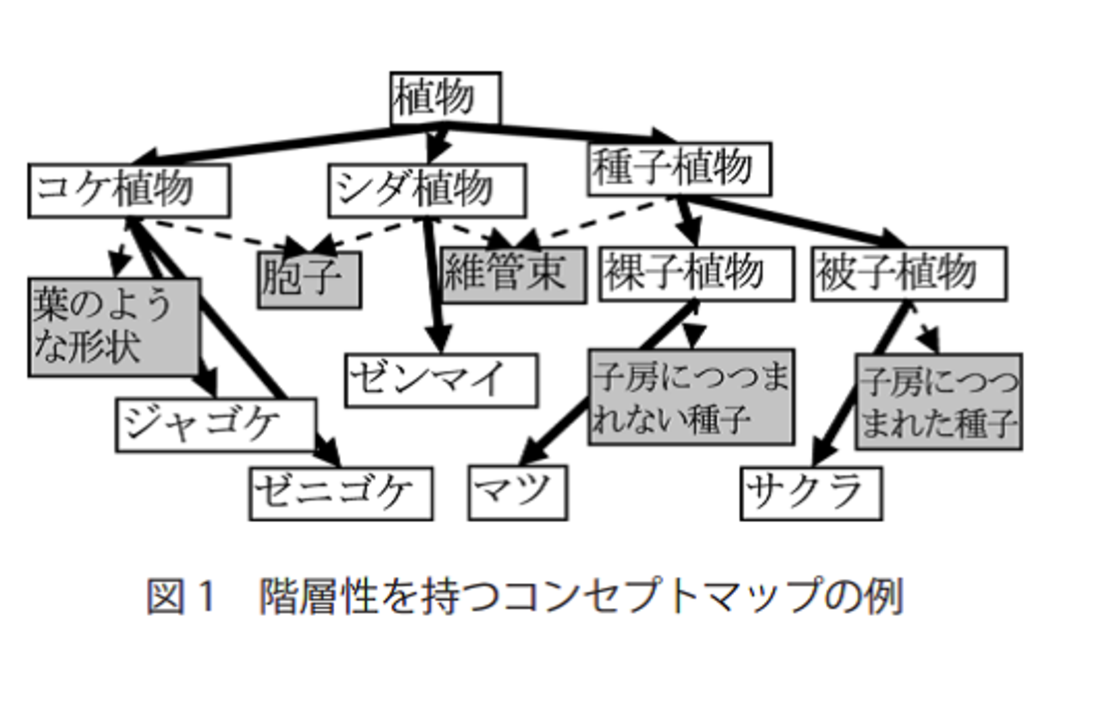
\includegraphics[width=8cm]{img/example_concept.eps}
\end{center}
\caption{コンセプトマップの例(出典: 誤りの可視化による階層構造の理解を指向したコンセプトマップ構築学習の支援環境 p.43 \cite{toumoto})}
\label{fig:example_concept}
\end{figure}

図\ref{fig:example_concept}は最上位の親を植物として,子にはコケ植物,シダ植物,種子植物が存在する,階層性のあるコンセプトマップである.
例えば種子植物に注目すると,その子である裸子植物,被子植物の間や,被子植物とサクラの間にも同様の親子関係が存在している.
また,コケ植物に注目すると,コケ植物には葉のような形状という独自の特徴すなわち属性を持っており,子であるジャゴケとゼニゴケにもその特徴は継承されている.
このようにして,コンセプトマップは概念間の関係性が可視化され,階層構造の理解に有効である.

一方コンセプトマップを学習の場で用いる場合大きく分け4つの形式が考えられる.
一つ目は,コンセプトマップを構築するテーマだけを与えられ,ノードとリンクを学習者が構築する形式.
二つ目は,コンセプトマップを構築するテーマと指導者側が学習者側に考慮してほしい概念をあらかじめ与えて,その他のノードやリンクを学習者に構築させる形式.
三つ目は,テーマとノードがすべて与えられて学習者はリンクのみを構築する形式.
四つ目は,テーマとあらかじめすべてのノードと一部のリンクが与えられ,残りのリンクのみを学習者が構築する形式.
本研究では,三つ目の形式で学習者にコンセプトマップを作成させた.


%
% キットビルド概念マップ
%
\chapter{キットビルド概念マップ}
\label{chap:kitbuild}
\section{本章の概要}
本章では,キットビルド概念マップについて述べる.
キットビルド概念マップ\cite{kit}\cite{kit2}は,教授者が内容理解構造として作成した概念マップを分解・部品化して学習者に提供し,学習者は提供された部品を組立てることで概念マップを作成する.
組立てられた概念マップは,元の概念マップと重畳することで差分抽出が可能であり,また,複数のマップの重畳することによる集団としてのマップ作成も可能となっている.
これによりキットビルド概念マップは,内容理解構造の全般的で直接的な表出と,評価の自動化を実現する手段として使われている.

以降,キットビルド概念マップの特徴について述べる.

\section{キットビルド概念マップの特徴}
授業理解の過程において,Kiewra\cite{kiewra}やArmbruster\cite{armbruster}は情報の取得と情報館付けによる構造化の二つの過程より成立するとした.
構造化の過程が理解に対してより重要であると分析している.
また,情報の取得に失敗した場合,構造化では補完できない場合が多いため,構造化対象となる情報を学習者に明示的に示し,学習者には構造化に注力させるべきであるとしている.
キットビルド概念マップでは,構造化の対象となる情報を部品として学習者に提供することによって,構造化を保持しつつ情報取得失敗時による構造化失敗を回避できるという特徴がある.

また,教材内容の理解を教授者が概念マップとして明示的に記述することが求められる.
このことから概念マップとして表現できない深い学習内容に対しては表面的な理解に留まるような形でしか表現できない.
しかし,深い学習内容に至る前提としてキットビルド概念マップで表面的な内容理解で使用できるという点ではキットビルド概念マップの有用性は損なわれない.

同様にして,教授者が適切な概念マップを作成できるとは限らず,また,唯一の正解である概念マップを作製できるわけではない.
しかし,キットビルド概念マップでは,教授者が作成した概念マップと学習者が作成した概念マップを比較し,形成的評価・フィードバックを受ける,
すなわち学習者が作成した概念マップにおいて再構成ができていない部分や,同様の誤りが多い部分が存在した場合,教授者側が作成した概念マップに誤りがあると考えられるという点から概念マップの修正を重ねてより正確な概念マップを作成できる.

以上のようにしてキットビルド概念マップには,学習者には学習内容の構造化に注力させ,その構造化自体に誤りがあったとしてもそれを修正していけるような形で作成されているマップであると言える.

%
% 関連研究
%
\chapter{関連研究}
\label{chap:refer}
\section{本章の概要}
本章では,本研究に関連する研究について述べる.
\ref{sec:concept_ref}節ではコンセプトマップを用いた研究について述べる.
\ref{sec:kasika_ref}節では学習成果の可視化に関する研究について述べる.
\ref{sec:my_thesis}節では,他研究と本研究にどのような違いがあるかを述べる.

\section{コンセプトマップを用いた研究}\label{sec:concept_ref}
コンセプトマップを用いた研究には,東本氏らの研究\cite{toumoto}と野村氏らの研究\cite{nomura_manabu}が挙げられる.
東本氏らの研究では,コンセプトアップを作成した学習者に対しフィードバックを返すことは重要であるが,決して容易ではないとしている.
第一に個別診断の困難性,第二に仮に診断をしても誤りをフィードバックしたとき,学習者の解答を否定し正解を提示する否定的フィードバックでは学習効果が低く,学習者はコンセプトマップの誤りを受け入れないか,なぜ誤りなのかを考えずに修正する可能性があり,自発的な誤り修正ができない点が挙げられる.
そこで,東本氏らは階層構造の理解の促進を目的とした学習者自身によるコンセプトマップの構築のためのシステム開発を行った.
特に,構築したコンセプトマップに対し,個別診断を行い,誤りがあれば誤りの可視化によるフィードバックを与えることとした.
東本氏らが提案した可視化手法は,各属性の意味を学習支援システムに組み込むため,汎用性が乏しいものとなった.
しかし,可視化を段階的に行うことにより,様々な階層性に対してもXMLや画像を用いれば可視化できるとしている.

野村氏の研究では,コンセプトマップはこれまで多くの教師が学校教育に取り入れており,コンセプトマップはある特定の学習過程において,教師と学習者が焦点化する必要のある少数のアイデアを明確にし,概念的意味を結びつける視覚的地図により,学習課題の達成後の図式的な要約を提供するものとしている.
しかし,コンセプトマップは学習中においても有効であるが最も友好的に利用できる可能なのは学習後の学習者の知識構成の表出であると主張している.
これはNovak\cite{concept}\cite{novak}が有意味学習の評価ツールとしてコンセプトマップが有効であるとしている点でも同様のことがいえるとしている.
そこで野村氏らはコンセプトマップを利用した学習ではなく,一定のまとまりのある学習内容を学習した結果をコンセプトマップを利用して評価することを想定とした,コンセプトマップを利用した学習評価支援システムを開発した.
このシステムでは,コンセプトマップの作成作業時間を短縮,管理を支援できる.

\section{学習成果の可視化に関する研究}\label{sec:kasika_ref}
学習成果の可視化に関する研究として,平塚氏ら\cite{hira}と手塚氏ら\cite{teduka}の研究が挙げられる.
平塚氏らの研究では,高等教育機関において学生自身が授業の学習成果を把握するものは,成績評定,GPA,資格取得などがあるとしているが,これらは授業単位を習得したという結果のみを計るものであり,学生にとって自分にどのような力が身についたのかわかりづらいとしている.
また,このことから学生は学習においての将来設計も難しくなり,授業の取り組みも消極的になるなど悪循環に陥ってしまう.
そこで,平塚氏らは学習成果の到達度を可視化し,学生に分かりやすい形で提示し自己効力感を得て学習意欲向上のために,教務システムとeポートフォリオを連携した学習成果可視化システムを構築した.
すでに同様のシステムを独自開発している事例はあるが,オープンソースのシステムを用いて構築し,公開・フィードバックする点が研究の意義としている.

手塚氏らの研究では,高等教育における振り返りは他者と関わりあいながら自主的に学び続けるために必要な能力として注目されているとし,構成主義的な学習観において教員が何を教えるかから学習者が何を学び取るかへと視点の転換が主張されていることから,学習中に期待通り成果が得られたのかどうかを常に振り返り,成功または失敗の要因を学習者が認識することが重要であるとしている.
しかし,全学習者が適切に振り返りを行えるとは限らないため,平塚氏らは振り返りの質的向上を目的とし,期末試験の予測得点と学習者データの可視化による振り返り支援システムを提案・開発した.
振り返りシステムでは,基礎数学の振り返りシートを分析し,eラーニングのヒント閲覧回数,eラーニングの学習時間,Vマーク式学習法におけるVの数が理解度の向上に結びつく振り返りに役立つことが考えられため,それらを折れ線グラフで時系列順に可視化するシステムを作成した.
これにより学習者は可視化機能を用いて学習でき,さらに各学習者がどのような学習データを見ながら振り返りを行っているのかというログが収集できる.

\section{本研究の特徴}\label{sec:my_thesis}
いままで上げてきた研究はどれも実際の授業の中でコンセプトマップや学習者の学習進捗を可視化しているものが多い.
一方,本研究では,eラーニングで学習する学習者に重きを置いている.
eラーニングは確かに授業の一環として用いられることもあるが,基本的には学習者一人で課題をこなしていくものが多い.
また,eラーニングにおけるフィードバックは否定的フィードバックが多く,何故間違えたのかという思考に至る可能性が低くなる.
加えて,今までの研究成果物はそのシステム上でのみ動作する物が多い.
本研究ではeラーニング上で学習する学習者に対して指導者が直接かかわらずとも学習者自身だけで,自身の学習理解度を把握し,学習目標を設定できる.
また,本システムはグラフデータの作成,削除や可視化に至るデータ取得に関して全てAPI化して実装している.
このことにより,本システムの可視化表現方法は本システムのみで使用できる機能となっているが,コンセプトマップの情報をグラフデータに変換し保存,削除,またデータ呼び出しに関してはAPIを通じて実行できる.
このことから,可視化に至るまでのデータ取得は任意のアプリケーションでも実施できるため,様々なeラーニングシステムで本システムの機能を実行できる.




%
% システム概要
%
\chapter{システム概要}
\label{chap:content}
\section{本章の概要}
本章では,本システムの概要について述べる.
本システムは,eラーニングで学習している学習者を対象としたシステムで,コンセプトマップを利用して学習者が学習目標を設定する場合に本システムを利用することを想定している.
本システムを利用して学習を進めることで,コンセプトマップにより自身の学習分野に対する構造的な理解を促進できるだけでなく,自身が進めている学習分野の主観的な知識獲得量を客観的に把握することが出来るため,学習目標を設定しやすくなる.

\ref{sec:kousei}節では,本システムの構成について述べる.
\ref{sec:env}節では,本システムの開発環境について述べる.
\ref{sec:about_system}節では,本システムにおける各機能の概要について述べる.
\ref{sec:futan}節では,本システムの運用における指導者の負担について述べる.

\section{本システムの構成}\label{sec:kousei}
本システムの構成を図\ref{fig:kousei}に示す.
本システムは,学習者がインターネットを通じて本システムのWebアプリケーションに接続することによってコンセプトマップを作成し学習を進めることができる.
本システムはすべての開発環境をDockerを用いて作成しているため,Dockerを使用できる環境であればどこでも本システムを実行することが可能である.

本システムで利用可能な学習教材は,その学習分野において教材提供者が階層構造を持つと判断した学習教材であれば利用可能である.
コンセプトマップを作成するにあたって,本システムではグラフデータベースを用いてコンセプトマップにおけるノードやリンク,リンクキーワードをグラフデータベースにおけるノード,エッジ,プロパティに変換することによってグラフデータベースにコンセプトマップのデータを保存し,その後グラフデータベースを可視化するライブラリを用いてコンセプトマップを閲覧,作成できる機能を作成した.
本システムを利用した学習手順として,学習者は指導者が作成した学習コンテンツを学び,そのフィードバックとして各問題がどのような学習分野となるのか教授してもらう.
その後,本システムを用いてそれぞれの学習分野をコンセプトマップを用いてどのような階層構造になっているのかを予測しながらコンセプトマップを作成する.
最後に本システムが指導者から入力された学習分野に対する階層構造のデータからコンセプトマップを自動的に作成する.
これにより学習者は,自身が作成したコンセプトマップと,自動的に作成されたコンセプトマップとを比較することにより,学習分野における自身の階層構造に対する理解を深めることができる.
加えて本システムではコンセプトマップのノードにおいて学習者の問題の回答情報から点数によってノードの背景色を表示できる.
これにより学習者は対象学習分野について,主観的に考えていた学習理解度と実際のテストの点数による学習理解度をはっきりと視覚的に確認でき,自分は特定分野においてしっかり学修できていたと思っていたが,実際はあまり理解できてきなかったという勘違いを正すことができる.
\begin{figure}[htbp]
\begin{center}
\includegraphics[width=10cm]{img/kousei.eps}
\end{center}
\caption{システム構成}
\label{fig:kousei}
\end{figure}

\section{開発環境}\label{sec:env}

\section{本システムにおける各機能の概要}\label{sec:about_system}

\section{本システムの運用における指導者の負担}\label{sec:futan}




%
% 学習者理解度可視化システム
%
\chapter{学習者理解度可視化システム}
\label{chap:system}
\section{本章の概要}
本章では,学習者理解度可視化システムとしてのシステムにおける具体的な実行手順と,実行手順の中で使用される機能についての詳細を述べる.

\section{システム実行の流れ}
\subsection{前提条件}
本システムを実行する前に満たすべき前提条件を示す.
まず,本システムは全てDocker上で動作するため,Dockerを使用できるPC上でのみ動作する.
そのPCの必要最低動作環境を表\ref{tab:docker_env}に示す.
\newpage
\begin{table}[htb]
    \centering
    \caption{Dockerのシステム要件}
    \label{tab:docker_env}
    \begin{tabular}{|c|c|}  \hline
        \multirow{5}{*}{Windows} & Windows 10 64 ビット:Pro、Enterprise、Education(ビルド 15063 以上) \\
		              & Hyper-V と Windows コンテナ機能の有効化 \\ 
                      & 64 ビット SLAT (Second Level Address Translation) 対応プロセッサ \\ 
                      & 4GB システムメモリ \\ 
                      & BIOS レベルでのハードウェア仮想化の有効化 \\ \hline
        \multirow{2}{*}{Intel チップの Mac} & macOS はバージョン 10.15 またはそれ以降 \\
        & 最小 4GB の メモリ RAM \\ \hline
        Apple silicon の Mac & Rosetta 2 のインストール \\ \hline
        \multirow{7}{*}{Linux系} & 仮想化のために、 64-bit カーネルと CPU のサポート \\
        & KVM 仮想化のサポート \\ 
        & QEMUバージョン5.2以上 \\
        & systemd init システム \\ 
        & Gnome または KDE デスクトップ環境 \\ 
        & 最小 4GB の メモリ RAM \\
        & ユーザ名前空間で ID マッピングの設定を有効化 \\ \hline
    \end{tabular}
\end{table}

以上の条件を満たすPC上でDockerをインストールすることにより,本システムは使用できる.
\newpage

\subsection{システム実行の流れ}
本節では,システム実行の流れについて説明する.
本システムの利用者は学習者とそれを指導する指導者となるため,両者それぞれのシステム実行の流れを説明する.
\subsubsection{指導者}
指導者は本システムを立ち上げて学習者が本システムを利用できるようにしなければならない.
まず,指導者は本システムをWebサーバーにインストールし,dockerコマンドを用いて本システムサーバを立ち上げる.
その後\url{http://127.0.0.1:7878/}にアクセスすることにより本システムにアクセスすることができる.
アクセスした直後のGUI(以下,ホーム画面)を図\ref{fig:home}に示す.

\begin{figure}[htbp]
\begin{center}
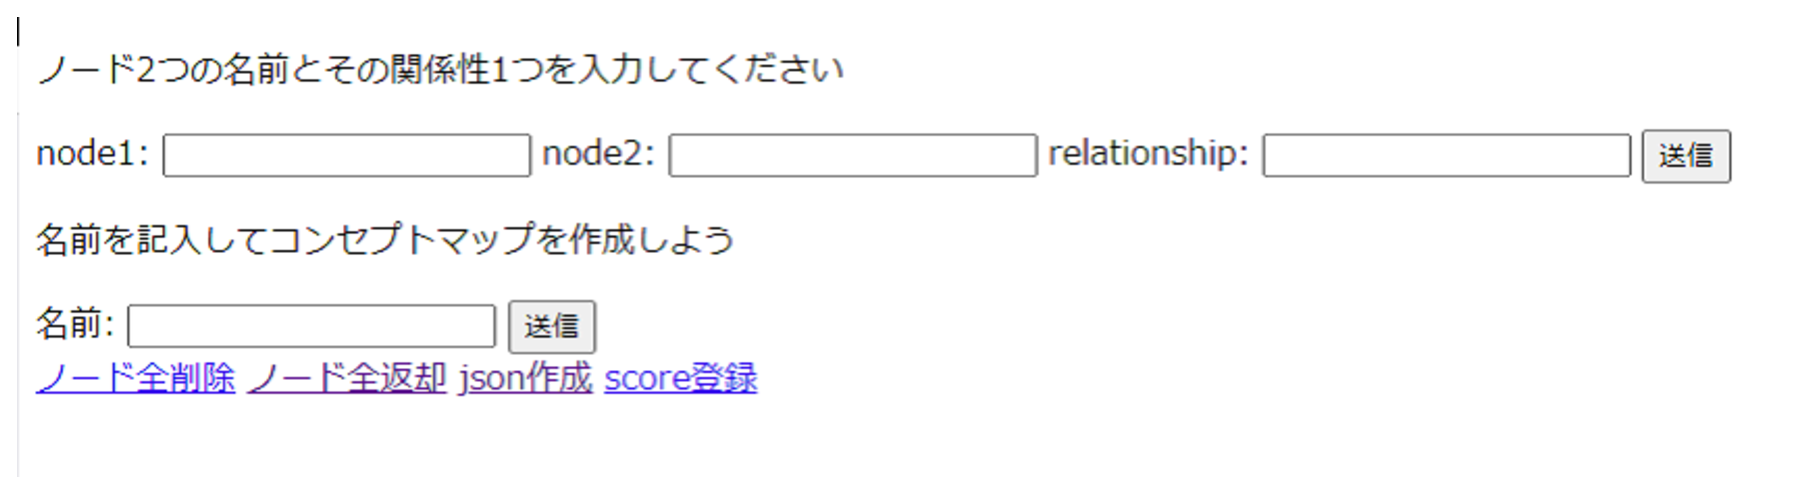
\includegraphics[width=18cm]{img/home.eps}
\end{center}
\caption{ホーム画面}
\label{fig:home}
\end{figure}

指導者はホーム画面のjson作成ボタンからグラフデータの入力を開始できる.
その後,第\ref{chap:content}章の\ref{subsec:hojo}節で示した図\ref{fig:hojo}のグラフデータ入力補助機能を用いてグラフデータを入力していく.
グラフデータの入力が完了した一例を図\ref{fig:ex_hojo}に示す.

\begin{figure}[htbp]
\begin{center}
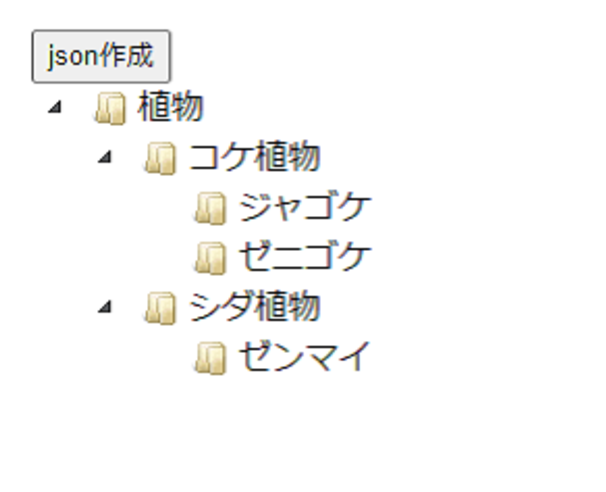
\includegraphics[width=10cm]{img/ex_hojo.eps}
\end{center}
\caption{グラフデータ入力一例}
\label{fig:ex_hojo}
\end{figure}

\newpage

グラフデータの入力が完了したらjson作成ボタンを押下する事により,グラフデータベースへデータの登録が完了する.
データが登録できたかどうかはホーム画面のノード全返却ボタンを押下して確認するか、\url{http://127.0.0.1:7474/}にアクセスすれば確認できる.
\url{http://127.0.0.1:7474/}にアクセスした際のGUIを図\ref{fig:neo4j_check}に示す.

\begin{figure}[htbp]
\begin{center}
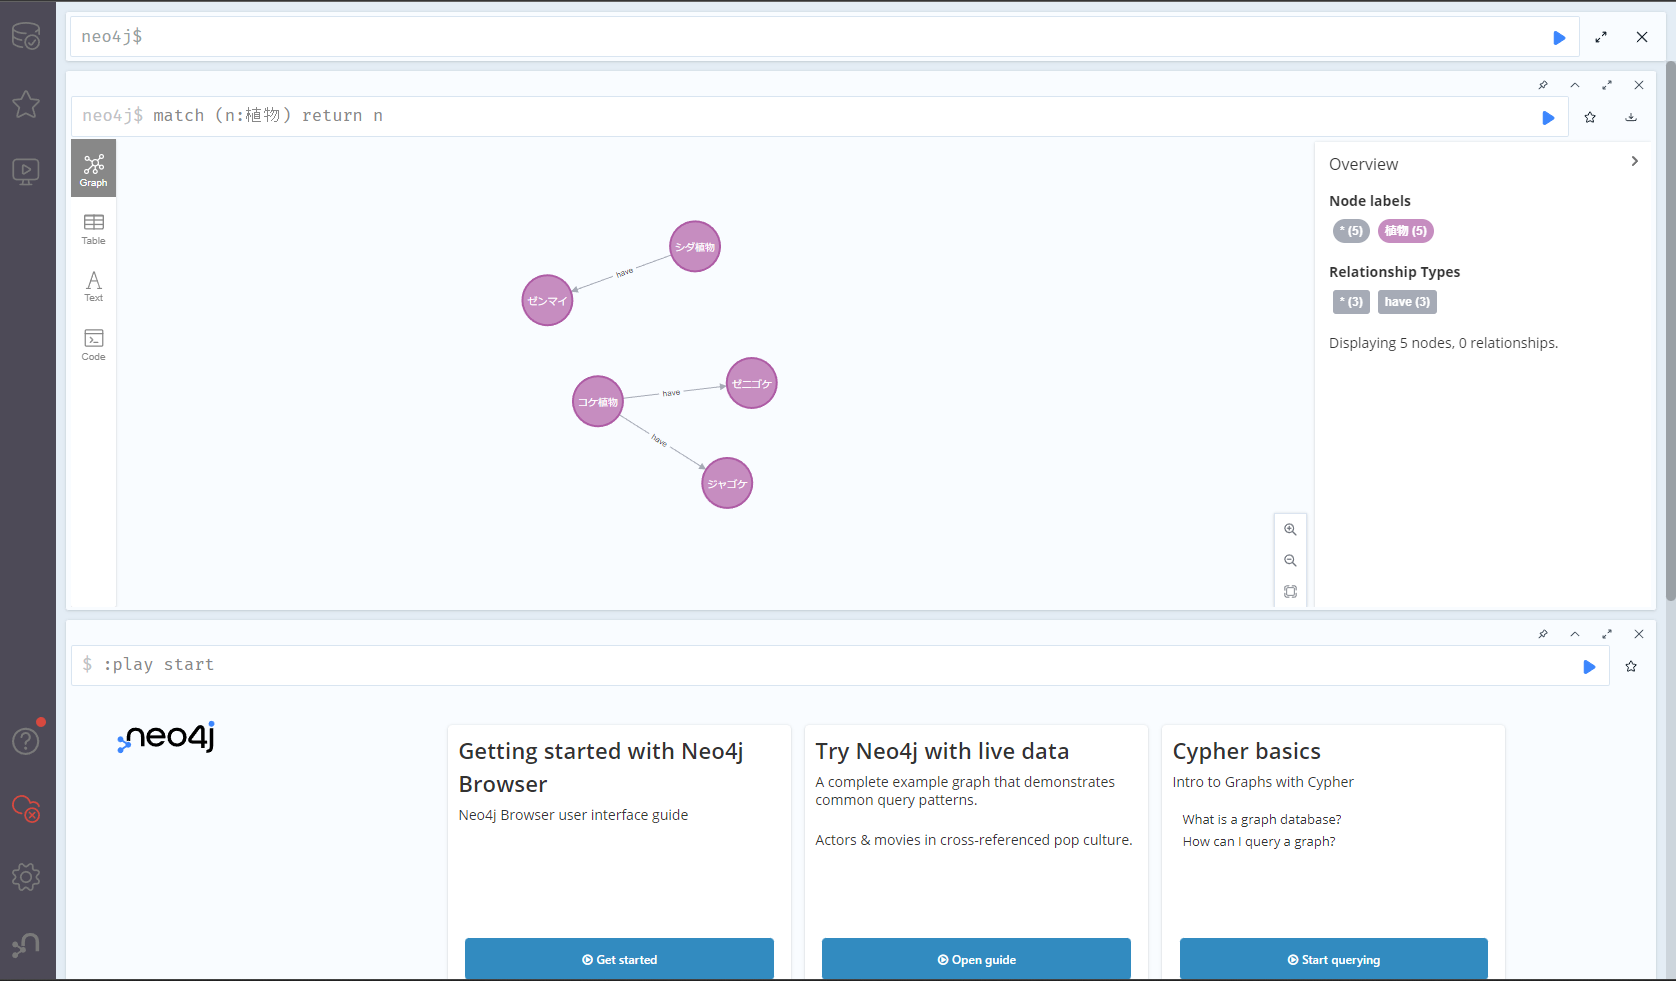
\includegraphics[width=18cm]{img/neo4j_check.eps}
\end{center}
\caption{グラフデータ確認画面}
\label{fig:neo4j_check}
\end{figure}
\newpage

図\ref{fig:neo4j_check}のページはNeo4jが提供するページで様々なクエリを発行することによってデータを閲覧できる.
今回はMATCH文を用いて先ほど入力したグラフデータを表示した.

続いて,グラフデータの入力が完了したら指導者は学習者に対して試験を実施する.
実施後の試験の結果を本システムに登録する必要がある.
登録するにはホーム画面のscore登録ボタンから学生の成績を登録できる.
score登録のGUIを図\ref{fig:score}に示す.

\begin{figure}[htbp]
\begin{center}
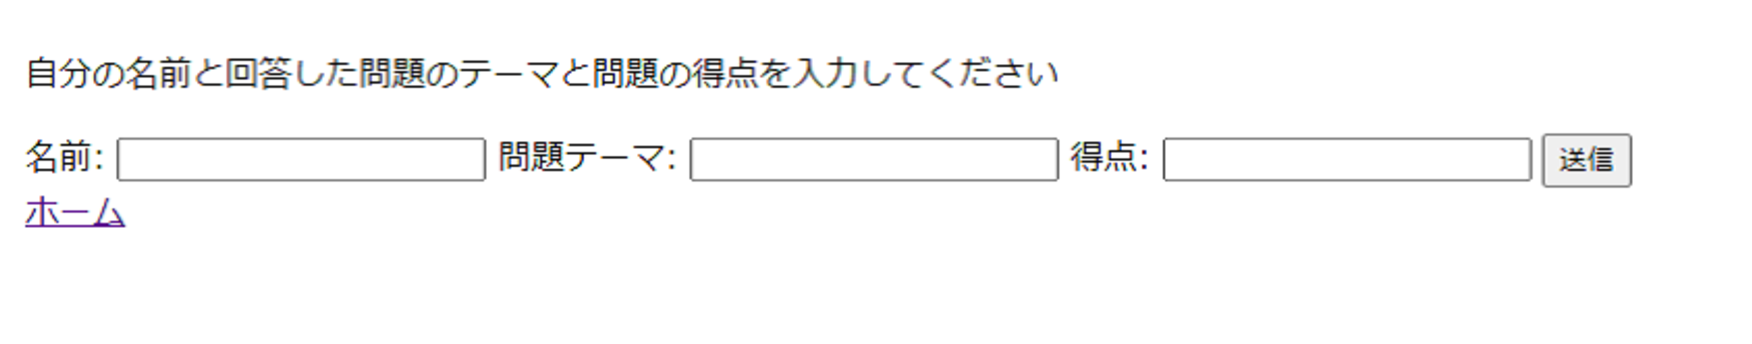
\includegraphics[width=18cm]{img/score.eps}
\end{center}
\caption{score登録画面}
\label{fig:score}
\end{figure}

このフォームでは名前の部分に学習者の名前を入力し,問題テーマに先ほど入力したグラフデータの子ノードに当たるものを入力し,得点を入力し,送信ボタンを押下することによって得点の登録が完了する.
例えば先ほど図\ref{fig:ex_hojo}で示したゼンマイの問題についてタケルという学習者が60点を取った場合は図\ref{fig:ex_score}のようにして入力する.

\begin{figure}[htbp]
\begin{center}
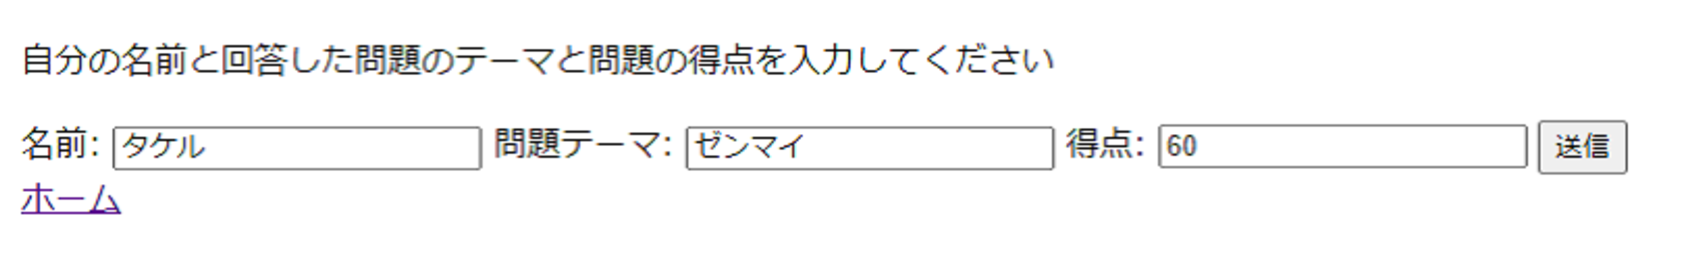
\includegraphics[width=18cm]{img/ex_score.eps}
\end{center}
\caption{score登録の一例}
\label{fig:ex_score}
\end{figure}
\newpage

\url{http://127.0.0.1:7474/}にアクセスしてデータを確認すると図\ref{fig:score_check}のようになっている.

\begin{figure}[htbp]
\begin{center}
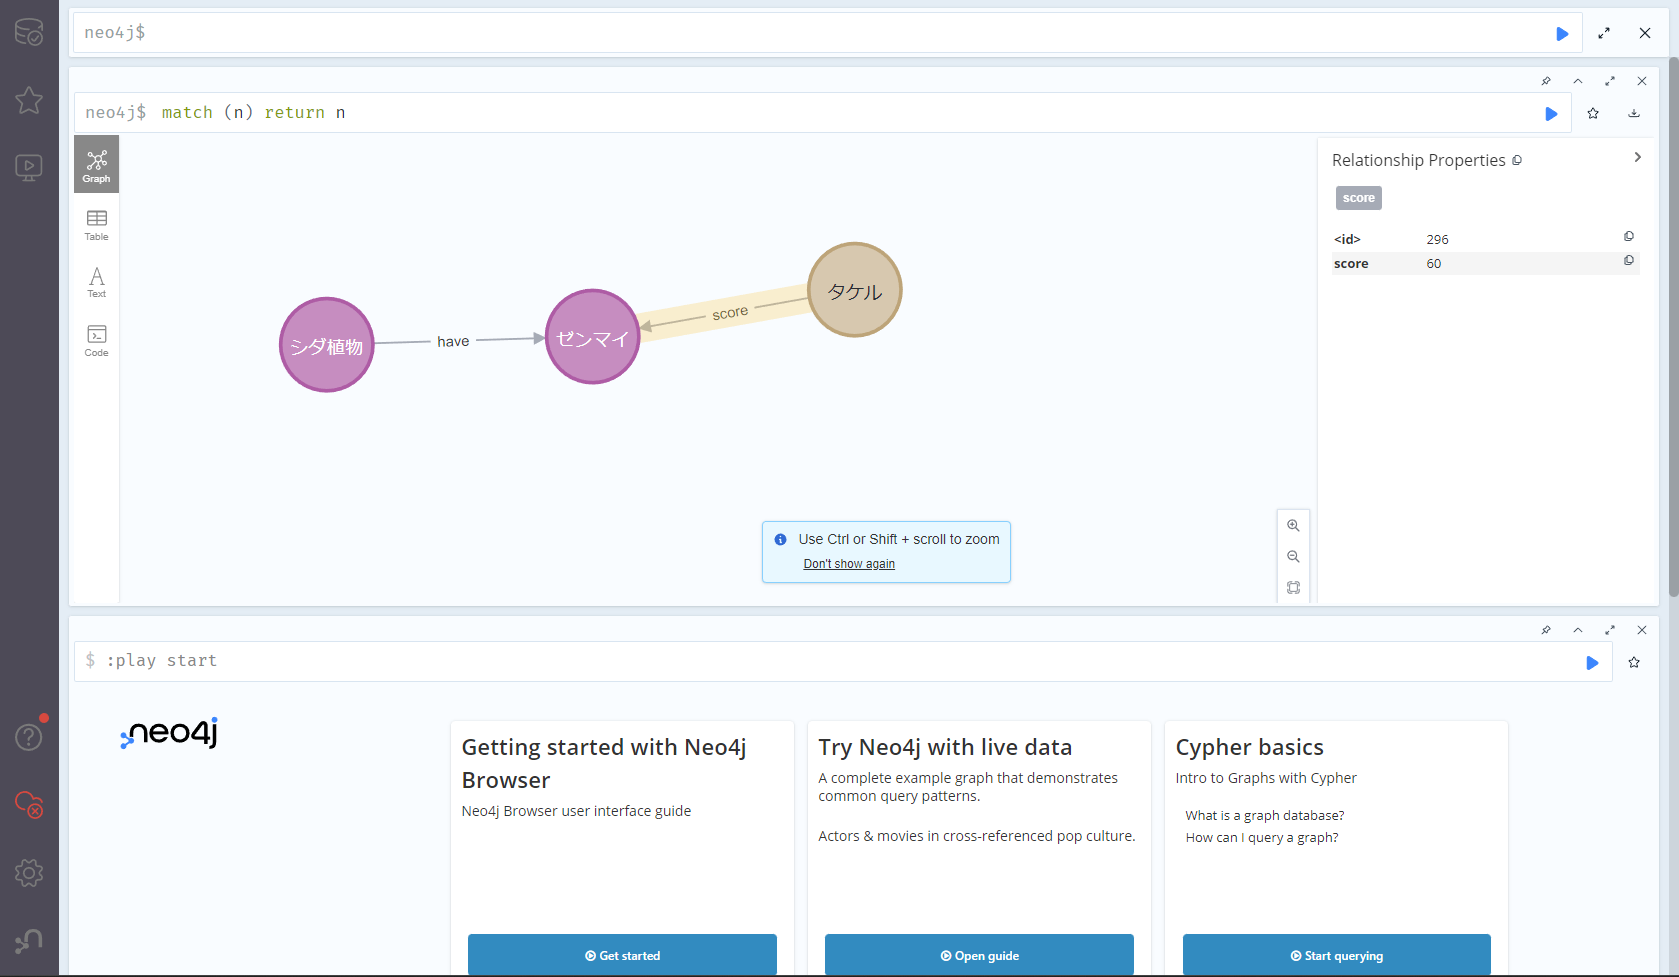
\includegraphics[width=18cm]{img/score_check.eps}
\end{center}
\caption{score登録の確認}
\label{fig:score_check}
\end{figure}
    
図で確認できるようにタケルがゼンマイに対してscoreを持っており,そのプロパティ内のscoreが60になっていることから先ほど入力した内容が反映されていることを確認できる.

以上の手順をもって,指導者はグラフデータの入力と学習者の成績登録を本システムで実施する.
\newpage

\subsubsection{学習者}
学習者はホーム画面の名前入力フォームに自身の名前を入力すればコンセプトマップ作成画面へと移行できる.
その一例を図\ref{fig:name_enter}に示す.

\begin{figure}[htbp]
\begin{center}
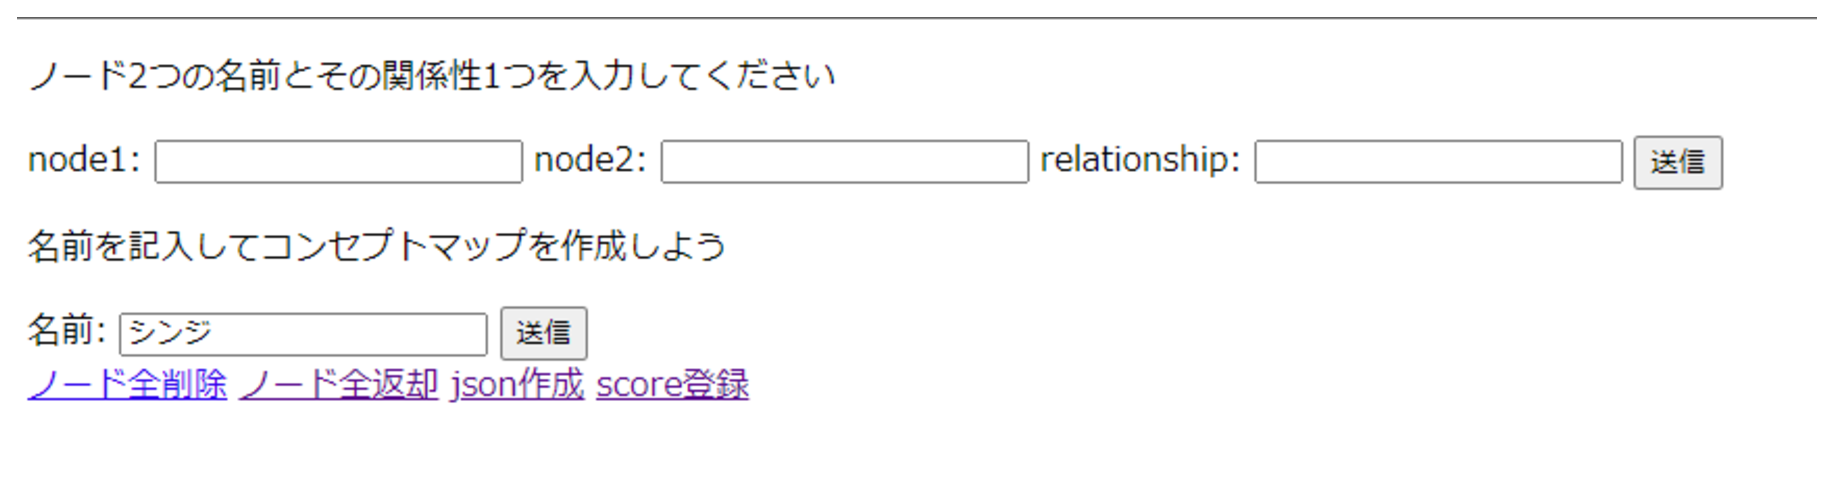
\includegraphics[width=18cm]{img/name_enter.eps}
\end{center}
\caption{名前入力画面}
\label{fig:name_enter}
\end{figure}

今回は例としてシンジという学習者が本システムを扱うこととしている.
名前入力後,シンジは図\ref{fig:sinji_concept}に示されたコンセプト作成画面へと移行できる.

\begin{figure}[htbp]
\begin{center}
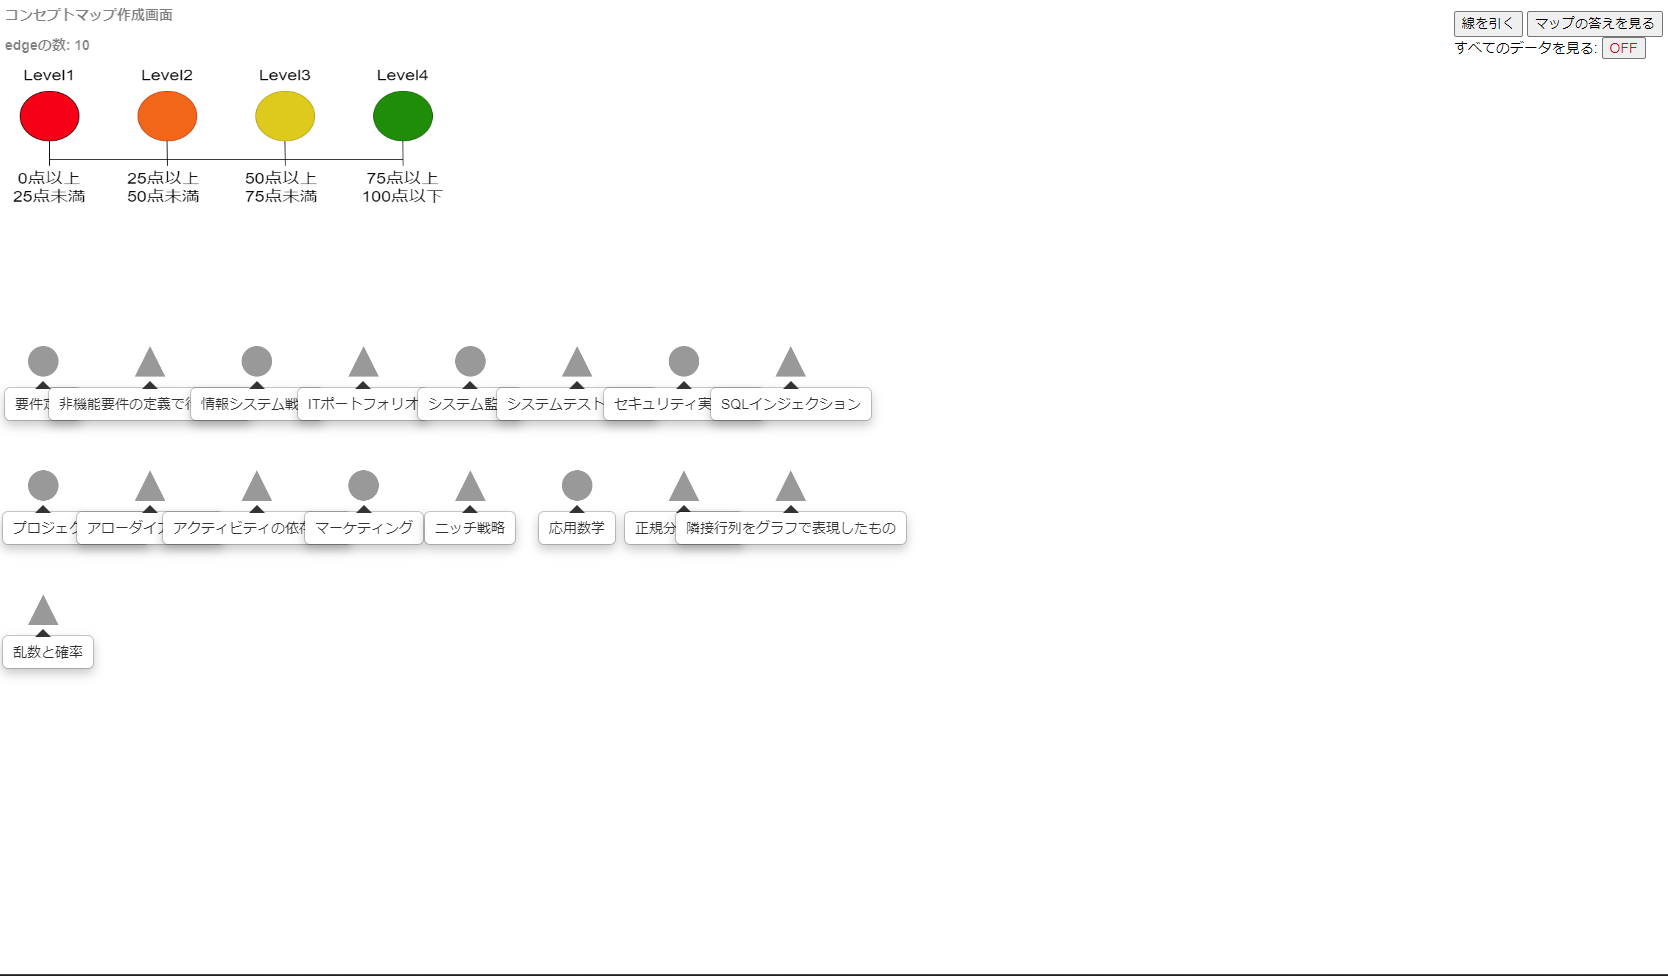
\includegraphics[width=14cm]{img/sinji_concept.eps}
\end{center}
\caption{コンセプトマップ作成画面}
\label{fig:sinji_concept}
\end{figure}
\newpage

コンセプトマップ作成画面遷移後,学習者は画面に表示されているノードを表す円と円とを結線機能を用いてノード情報を確認しながら結線していく.
結線する数はedgeの数で確認し,結線する場合は画面右上の「線を引く」ボタンを押下することによって結線ができる状態に移行する.
学習者は自分が思うコンセプトマップを作成していき,最後に試験の主観的獲得点数量に基づいて,ノードをタップすることによってノードの背景色を変更できる.
背景色は獲得点数の割合が 0\%以上 25\%未満なら赤,25\%以上 50\%未満なら橙,50\%以上 75\%未満なら黄,75\%以上 100\%以下なら緑と設定できる.
背景色決定後,画面右上の「マップの答えを見る」ボタンによりコンセプトマップの答えを確認できる.
その様子を図\ref{fig:sinji_check}に示す.

\begin{figure}[htbp]
\begin{center}
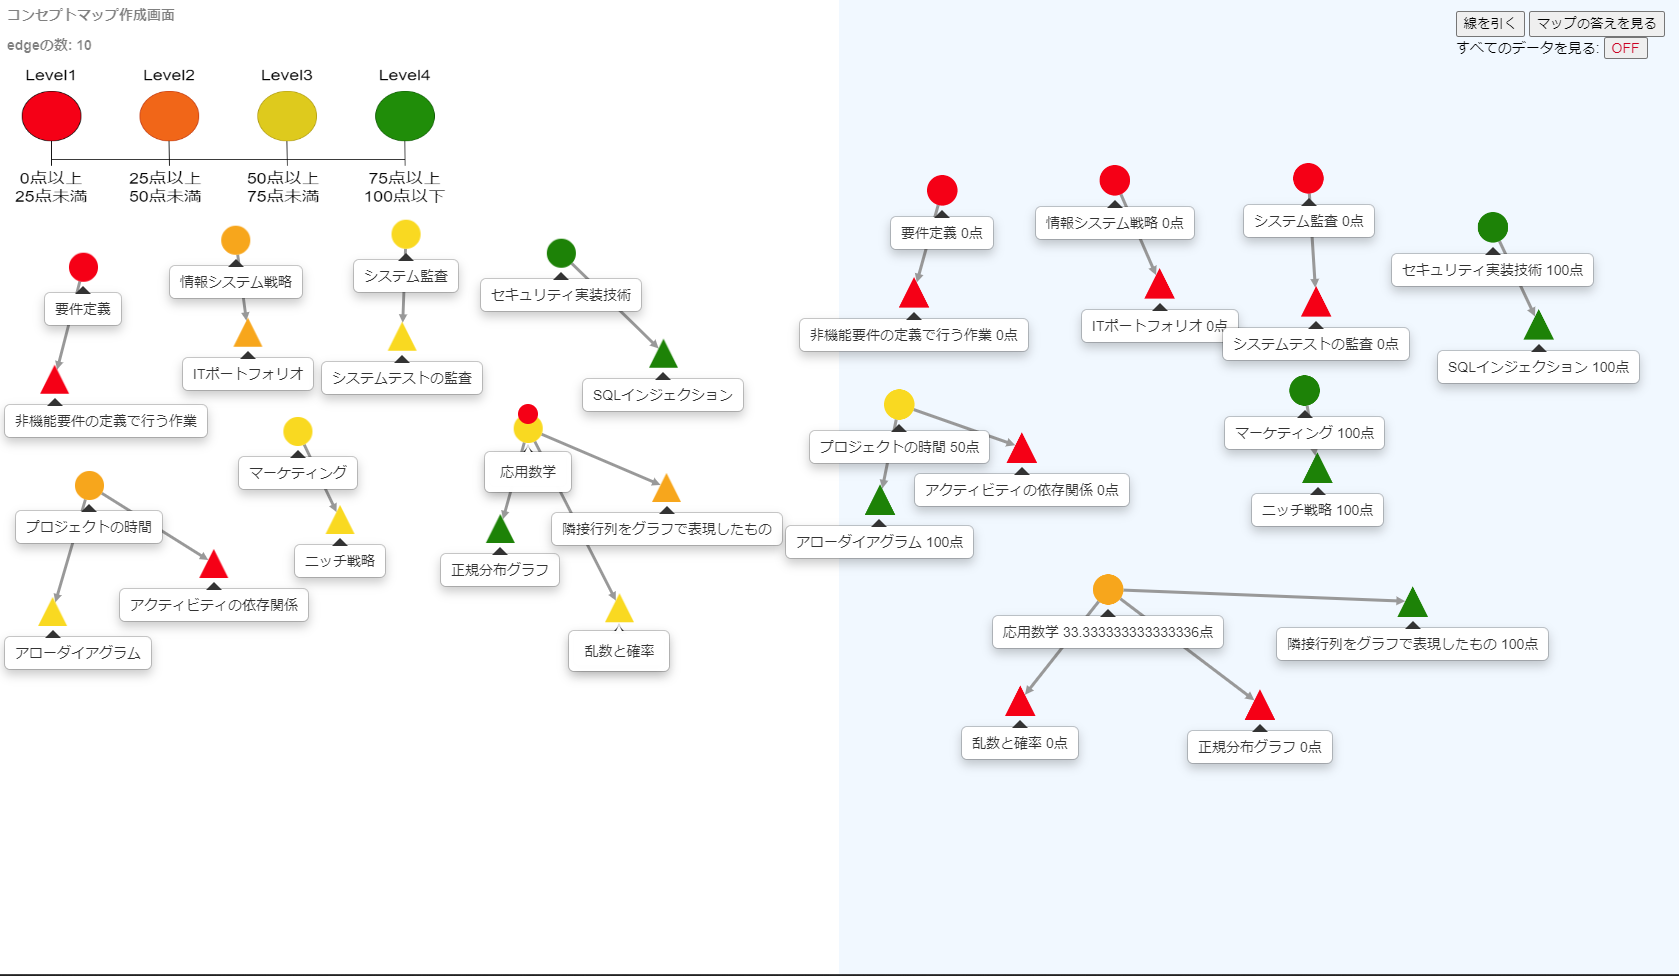
\includegraphics[width=18cm]{img/kasi_system.eps}
\end{center}
\caption{コンセプトマップ確認のGUI}
\label{fig:sinji_check}
\end{figure}
\newpage

学習者はコンセプトマップ比較時に表示されているデータが邪魔であれば画面右上のすべてのデータを見るボタンを押下することによって,データの表示と非表示を選択できる.
また,ノードにマウスを重ねると一つ一つのノード情報を確認することもできる.
これらの機能を駆使して学習者は自身が作成したコンセプトマップと,システムが自動的に作成したコンセプトマップを比較することにより,
コンセプトマップの誤りがあればそれを修正し,続いてノードの背景色を比較し,自身のその分野に対する学習理解度において認識の齟齬があるかを確認し,誤りがあれば修正していく.

以上の作業で学習者は,自身が学ぶ学習分野において学習構造と学習理解度をコンセプトマップとノードの背景色をもって客観的に自身の学習理解度を認識できるため,学習目標設定の基準にできる.


%
% 評価実験
%
\chapter{評価実験}
\label{chap:experiment}
\section{本章の概要}
本章では,開発したシステムの評価実験とその考察について述べる.
そして本研究では,学習者が座学における学習目標設定方法による学習と本システムのグラフデータ可視化機能を用いた学習目標設定方法による学習を比較し,
有用性を検証するための事前事後テストによる評価実験とアンケートによる利用評価実験を実施した.

\section{座学と比較した本システムによる学習の有用性検証実験}
実験では,基本情報技術者試験の午前試験を基にした,事前テスト事後テストによる座学と比較した本システムによる
学習の有用性を検証した.

\subsection{実験対象者}
実験対象者は,情報学科の学生と情報学科を卒業した大学院生(4年生:4名,修士1年生:7名,修士2年生:5名)の16名を実験協力者とした.
当学科では,3年生までにプログラミングは勿論ながら様々な情報学に関しての講義があるため,基本情報処理技術者試験の午前試験に関する知識も備えている.

\subsection{実験準備}
本実験を実施するにあたり,基本情報技術者試験の午前試験に関する事前テスト・事後テストを用意した.
学習教材としては事前テストに解説を付属させておりそれを学習教材とした.

事前テスト,事後テストはともに10点満点として,事前テスト・事後テストは同レベルの別の問題を使用した.
事前テストと事後テストはGoole From上で解答してもらった.
事前テストの内容を図\ref{fig:jizen1}~図\ref{fig:jizen5}に示す.
事後テストの内容を図\ref{fig:jigo1}~図\ref{fig:jigo5}に示す.
学習教材の例を図\ref{fig:kyozai1},図\ref{fig:kyozai2}に示す.


%
% 結論
%
\chapter{おわりに}
\label{chap:conclusion}
e ラーニング上で学習するにあたり,自身の学習目標を設定することは,学びを深める手段のうちの一つである.
一方,学習目標を設定するには,自身が学習したい対象の知識を把握している必要がある.
しかし,学習者自身では学習項目を理解していると主観的には考えていても,他人が客観的に判断すると理解できていない場合があり,学習者自身で学習目標を設定することは必ずしも容易ではない.

そこで本研究では,学習目標の設定支援を目的に,学習者の理解度を可視化する,グラフデータベース を用いた学習者理解度可視化システムを開発した.
本システムは e ラーニングで学習している学習者を対象としたシステムで,コンセプトマップ(以下,CMap)を利用して学習者が学習目標を設定する場合に本システムを利用することを想定している.
学習者は指導者が作成した問題を解き,本システムを用いてCMapを作成する.
本システムでは学習者の回答情報からCMapを作成し,学習者は自身が作成したCMapと,システムが生成したCMapを比較することにより,自身の学習理解度を客観的に確認でき,学習目標設定の基準にできる.

開発した本システムを評価するために,学習者が座学における学習目標設定方法による学習と本システムのグラフデータ可視化機能を用いた学習目標設定方法による学習を比較し,有用性を検証するための事前事後テストによる評価実験とアンケートによる利用評価実験を実施した.
座学と比較した本システムによる学習の有用性検証実験では,情報学科の学生と情報学科を卒業した大学院生16名に対して基本情報技術者試験の午前試験を基にした,事前テスト事後テストよる座学と比較した本システムによる学習の有用性を検証した.
結果として,座学すなわちシステム非利用者群の事前テストと事後テストの平均点が0.75 点増えているのに対し,本システム利用者群の平均点は2.125 点上昇していた.
このことから,座学で学習したシステム非利用者群と比較して,本システムを利用して学習したシステム利用者群の方がより高い点数が得られたことが確認できた.

また,本システムの利用評価実験では,システム利用者群はシステム非利用者群と比べて,自分の主観的学習理解度と実際に返却された学習理解度に差がなかったことが表されている.
すなわち,システム利用者の方がシステム非利用者と比べて,学習者自身の学習内容に対する主観的理解度と客観的理解度に差がなかったことが分かった.
この結果から,システム利用者群は正しく自身の学習進行度を理解できていたため,システム非利用者群より事後テストの得点が上昇していたのではと考えられる.

本研究では,e ラーニングにおける学習目標設定支援を目的に,学習者の理解度をCMapで可視化する,グラフデータベースを用いた学習者理解度システムを開発した.
実験の結果座学で学習したグループと比較して,本システムを利用して学習したグループの方がより有意に点数が高いことが確認できた.
このことから本システムは学習目標設定支援が可能である.

%
% 謝辞
%
\acknowledgement % \chapter*{謝辞}
\addcontentsline{toc}{chapter}{謝辞}
本論文は近畿大学大学院総合理工学研究科エレクトロニクス系工学専攻においての研究成果をまとめたものである.

本研究を遂行するに当たり,熱心な御指導および御鞭撻をいただきました指導教員である近畿大学情報学部の井口信和教授,近畿大学情報学部の越智洋司准教授,近畿大学情報学部の山元翔講師に深く感謝の意を表します.

論文審査にあたり,主査を担当して下さいました近畿大学情報学部の越智洋司准教授,副主査を担当して下さいました近畿大学情報学部の森山真光准教授に心より御礼申し上げます.

%
% 参考文献
%
\chapter*{参考文献}
\addcontentsline{toc}{chapter}{参考文献}
\bibliography{references} %references.bibから拡張子を外した名前
\bibliographystyle{junsrt} %参考文献出力スタイル

%
% 研究発表
%
\chapter*{研究発表}
\addcontentsline{toc}{chapter}{研究発表}
\begin{flushleft}
    1.\underline{栗岡陽平},井口信和: “動的ドリルを用いた e ラーニング問題作成支援システムにおける学習者の理解度評価に関する考察”,2021年度 情報処理学会関西支部 支部大会,2021年9月19日(オンライン)
    \end{flushleft}
    
    \begin{flushleft}
    2.\underline{栗岡陽平},山元翔,越智洋司,井口信和: “グラフデータベースを用いた学習者理解度可視化システムの提案”,情報処理学会第84回全国大会,2022.3.3~2020.3.4(オンライン)
    \end{flushleft}

    \begin{flushleft}
    3.\underline{栗岡陽平},山元翔,越智洋司,井口信和: “グラフデータベースを用いた学習者理解度可視化システムの開発”,理工マスターズ,2022.5.21(近畿大学東大阪キャンパス)
    \end{flushleft}

    \begin{flushleft}
    4.\underline{栗岡陽平},山元翔,越智洋司,井口信和: “グラフデータベースを用いた学習者理解度可視化システムの開発”,第47回 教育システム情報学会全国大会,2022.8.24~2022.8.26(オンライン)
    \end{flushleft}

    \begin{flushright}
    以上
    \end{flushright}

%
% % 付録
% %
% \chapter*{付録}
% \addcontentsline{toc}{chapter}{付録}
% \appendix
\section{付録について}
本研究で作成したプログラムのソースファイルなどを卒業研究報告書に含めた
い場合は,付録として巻末にまとめておく.

\end{document}